%!TEX root = ../Montravail.tex

\chapter{Language Syntax}
%\addcontentsline{toc}{chapter}{Grundlagen}
\lhead[ \leftmark   ]{\textbf{Language Syntax}}

%erstes Unterkapitel
\section{express structural concepts}

\textcolor[rgb]{1,0,0}{Why do we need a description?
? Designers: to communicate ideas
? Implementors: to build a conforming compiler
? Programmers: how do I write a while loop in language X?}

%n�chstes unterkapitel ebene 2
\subsection{features to describe}
? syntax: legal sentences
? semantics
? static: checked at compile time
? dynamic: run time behaviour\\\\
a simple, compact and unambiguous notation:
? We need a formal description rather than an informal (natural) language
description.
%n�chstes unterkapitel ebene 2
\subsection{Zweite �berschrift}
the ASCI character version\\\\
lexems identifiers and strings
numbers are built-in primitive symbols

%unterkapitel Ebene 3 nicht im Inhaltsverzeichnis aufgef�hrt! 
\subsubsection{the language evolution}
\textit{hier kann Kursiv geschrieben werden}
xy were sentences and equals was a verb
xy are nouns and equals is an operation
Just as the noun yx names the ...
Many people think of all mathematical expressions as sentences, reading 1+1
as Add 1 and 1. They think of 1 + 1 = 2 as asserting
%zweites Unterkapitel
\section{Well-writen}
how to write a module?
%n�chstes unterkapitel ebene 2
\subsection{qualities}
written in a declarative style that has the goal of making
%Abbildungsbeispiel
%Abbildungsquelle immer! angeben es sei den selber gemacht!!!!
Text....(siehe Abb. 1.1)

\begin{figure}[!ht]
	%mitte der Seite
	\centering
		%[nat�rliche Breite in Pixeln, nat�rliche H�he in Pixeln, Abh�ngigkeit von der Textbreite]
		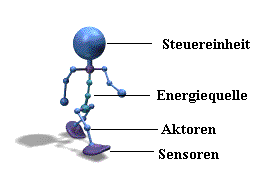
\includegraphics[natwidth=1200pt, natheight=349pt, width=0.4\textwidth]{grafiken/Robotpeintre.PNG}
	\caption[Aufbau allgemein]{Aufbau und Komponenten von Robotern}
	\label{fig:Aufbau und Komponenten von Robotern}
\end{figure}

\subsection{TLA+}
%unterkapitel Ebene 3 nicht im Inhaltsverzeichnis aufgef�hrt!
\subsubsection{Propositional logic is the study of simple operations on Booleans (truth values)}
all the opssilies tha can occur , as probabilitee
all the cases that can be defined with the semantic
%Aufz�hlung
\begin{itemize}
	\item introduce an extra level of indirection between your domain abstraction and the lan
	guage of implementation.
	\item  extensible abstractions 
	\item Die Formen des Arbeitsraums
\end{itemize}
    
... extensible abstractions. (Vgl.\cite{112})
as a manager translates the sentence into a set of separate sentences, checks the ones that are trivially true, and sends the others to one
or more other ...\\\\
manager remembers if it has already .. an .. \\\\
This would be inelegant but feasible\\\\
 being completely rigorous
and using the notation of dsl2ttcn3 , you would have to write G[1] and G[2] instead
of N and E . (If you were restricted to ordinary dsl notation, you would
have no way to be rigorous.)\\\\
%n�chstes unterkapitel ebene 2
\subsection{implementation inheritance}
%unterkapitel Ebene 3 nicht im Inhaltsverzeichnis aufgef�hrt!
\subsubsection{Dritte �berschrift}
dsl in action\index{A.2.2 Subtyping to prevent implementation leak}
\textcolor[rgb]{1,0,0}{subclasses become unnecessarily coupled to the implementation of your base class!
how to distill an abstraction out of its nonessential details
minimize accidental complexity in your abstractions}
%� ohne weiterf�hrung des Wortes
Roboterfu\ss \ befindet

homogene\\ 4 x 4  Matrix:

\begin{equation} 
T = \begin{pmatrix}
     Ax&Ay&Az&0\\Bx&By&Bz&0\\Cx&Cy&Cz&0\\Px&Py&Pz&1
     \end{pmatrix}
\end{equation}


\begin{equation}(\theta, d, a, \alpha)\end{equation}
 
verschiedene Matrizen:

\begin{equation}
T=\begin{pmatrix}\cos\theta & -\sin\theta \cos\alpha & \sin\theta \sin\alpha & \arccos\theta\\ \sin\theta & \cos\theta \cos\alpha & -\cos\theta \sin\alpha & \arcsin\theta\\ 0 & \sin\alpha & \cos\alpha & d\\ 0 & 0 & 0 & 1\end{pmatrix}
\end{equation}

\begin{equation}
^{n - 1}T_n
  = \begin{pmatrix}
    \cos\theta_n & -\sin\theta_n \cos\alpha_n & \sin\theta_n \sin\alpha_n & a_n \cos\theta_n \\
    \sin\theta_n & \cos\theta_n \cos\alpha_n & -\cos\theta_n \sin\alpha_n & a_n \sin\theta_n \\
    0 & \sin\alpha_n & \cos\alpha_n & d_n \\
    0 & 0 & 0 & 1
  \end{pmatrix}.
\end{equation}


\begin{equation}
T=T_1T_2T_3T_4T_5T_{tcp}
\end{equation}


%Beispiel f�r eine Tabelle
Text...(Siehe Tab. 1.1)
\\\\
\textbf{Titel:}\\%Der Titel bei Tabellen muss immer �ber der Tabelle stehen Statuten FH-Koeln! bei Abbildungen drunter! 
\begin{table}[ht]
\centering
\caption[Titel]{Titel}	
	 \begin{tabular}{|c|p{11cm}|}
			\hline
			\rowcolor{sourcegray}
			\textbf{�berschrift 1} & \textbf{�berschrift 2}\\
			\hline
			Text & Text \newline 
						 Text\\
			\hline
			Text & Text \newline 
						 Text\\
			\hline
		\end{tabular}
	\vspace{1.0em}
	%\caption[Mobilit�tsgrade]{Gliederung der Mobilit�tsgrade}
	\label{tab:Titel}
\end{table}

\newpage
%erstes Unterkapitel
\section{The process of writing a correct specification }

\textcolor[rgb]{1,0,0}{This is a procedure I use regularly when writing code that is at all tricky and that I want to be correct. But, getting this program correct was not important
enough to warrant spending that much time. ???}

%n�chstes unterkapitel ebene 2
\subsection{features to describe}
most obviously correct specifications could not be executed efficiently
The thing to do in such a case is to write two versions of some definitions:
one that is simpler and more obviously correct, and another that dsl can evaluate more efficiently.
%n�chstes unterkapitel ebene 2
\subsection{Sorting the elements of the specification}


We want to specify what it means to sort a set of elements. For simplicity, let?s
assume that each element is a record ? * with a key component, and the elements
are to be sorted in increasing order of their key value.
Sorting a set means arranging its elements in a list. A sorting of a set S is
therefore a list of elements of S that contains each element exactly once and is
sorted according to the elements? key values. To describe this precisely, we must
define:
? What a list of elements of S is.
? What it means for such a list to contain each element of S exactly once.
? What it means for the list to be sorted according to elements? key values.
\\\\
However,
if she defined a Turing machine T to be a 7-tuple, it would be impossible to
remember if its initial state was T [4] or T [5]. Programming languages solve this problem by introducing records.\\\\
the record\\\\
*Records in Programming Languages
A record is called a struct in the C programming language. In more modern
programming languages, an object is a record for which certain operations are
defined. In addition to using r .f to mean the value of field f of record r ,
these languages also use r .O(. . .) to mean the value obtained (and side effects
produced) by appying the operation O to the record r .
If you program in an object-oriented language, you may miss some of its fea-
tures when using TLA + . While those features are useful for writing programs,
they are not needed for writing specifications, and their inherent mathematical
complexity would make specifications that used them harder to understand.

%n�chstes unterkapitel ebene 2
\subsection{The Hierarchical Structure}

To write the spec, I had to decide how to represent the voters?
ballots. The obvious way to represent a single voter?s ballot is by a sequence
whose i th element is the name of the candidate the voter ranks number i . An
obvious way to represent all the votes is as a set of such sequences. However,
that?s not right because two voters can cast identical ballots, and there is no
concept of a set having ?two copies? of an element. Here are three reasonable
ways to represent the collection of votes:
? With a set whose elements are records or tuples with one component being
the ranking and the other identifying the voter (with a randomly chosen
identification if the vote is to be anonymous).
? With a bag (multiset) ? of rankings.
? With a sequence of rankings, arranged in an arbitrary order.
%n�chstes unterkapitel ebene 2
\subsection{System as a formula}
diferent specifications lead to the same Module definition
one standard interpretation

%unterkapitel Ebene 3 nicht im Inhaltsverzeichnis aufgef�hrt!
\subsubsection{Writing Structured specifications}
dsl in action\index{A.2.2 Subtyping to prevent implementation leak}
\textcolor[rgb]{1,0,0}{A module consists of module definition describing the module, followed by either:
Writing Structured optional module control part
? A non-module control that is a sequence of steps, ending with a qed step, each of which may (but need not) have a control part.
? A module control, which is either the keyword obvious, the keyword omitted, or a by ....}

after\\\\
conjunction... formula like tla+



\newpage
%Beispiel f�r zwei Bilder nebeneinander
\begin{figure}[!ht]
\centering 
\begin{minipage}[hbt]{7cm}
	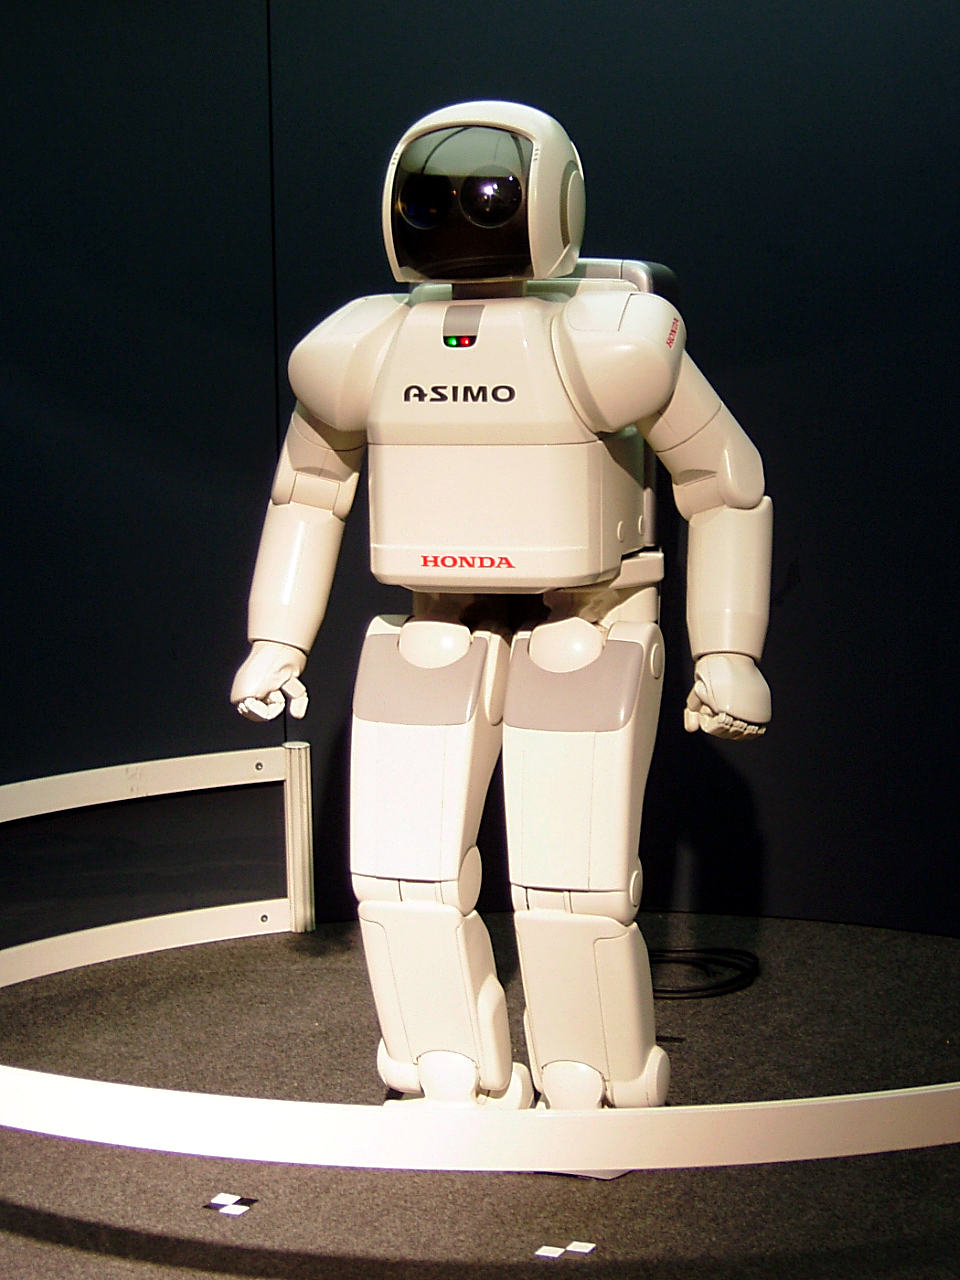
\includegraphics[width=7cm]{grafiken/HONDA_ASIMO.jpg}
\end{minipage}
\begin{minipage}[hbt]{6.7cm}
	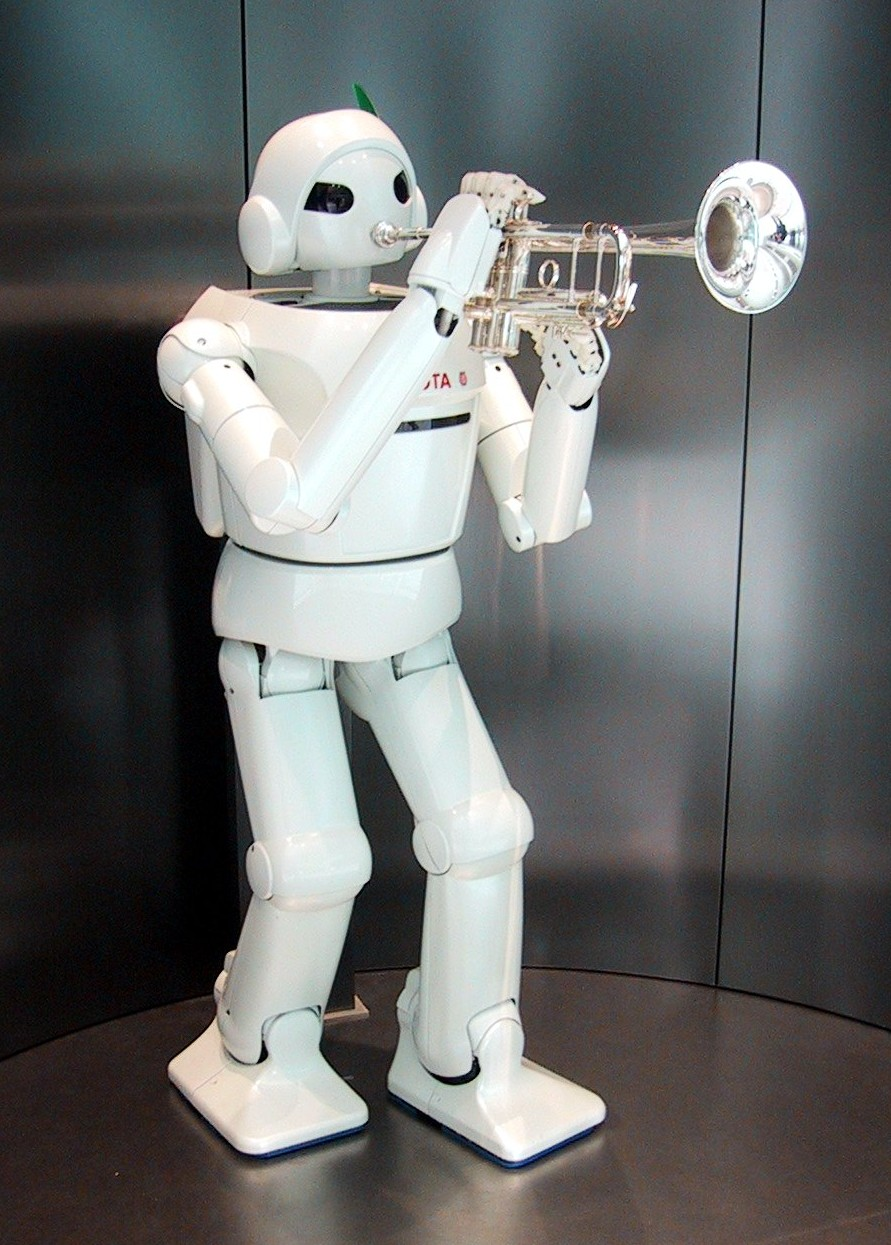
\includegraphics[width=6.7cm]{grafiken/Toyota_Robot_at_Toyota_Kaikan.jpg}
	\end{minipage}
	\caption[Humanoide Roboter]{Humanoide Roboter Links der Aibo von Honda rechts der Roboter von Toyota}
	\label{Humanoide Roboter}
\end{figure}

Bild-Quellen:(\url{http://de.wikipedia.org/wiki/Humanoider_Roboter})\\Sichtung: 17.09.2010\\\\

In Abb. 1.2 sind...Text\\\\
 
%�bersichtshalber besser Begriffe betonen
Kraft \textbf{F}, der Masse \textbf{m} und der Beschleunigung \textbf{a} kann mit der daraus resultieren Formel die Kraft, die wirkt, berechnet werden: \begin{equation}F = m * a \end{equation} Folglich ist die Kraft das Produkt von Masse und Beschleunigung.  

%Formeln 
SI-Einheit der Kraft:
\begin{equation}
[F] = kg * \frac{m}{s^{2}} = Newton (N)
\end{equation}

\begin{equation}M = F * l = F * r * \sin\alpha \end{equation}
 
SI-Einheit des Drehmomentes: \begin{equation}[M] = Newtonmeter (N * m)\end{equation}
 